\chapter{Diseño}

\section{Introducción}
En este capítulo 

\subsection{Diseño de interfaces de usuario}


\begin{figure}[H]
    \centering
    \centerline{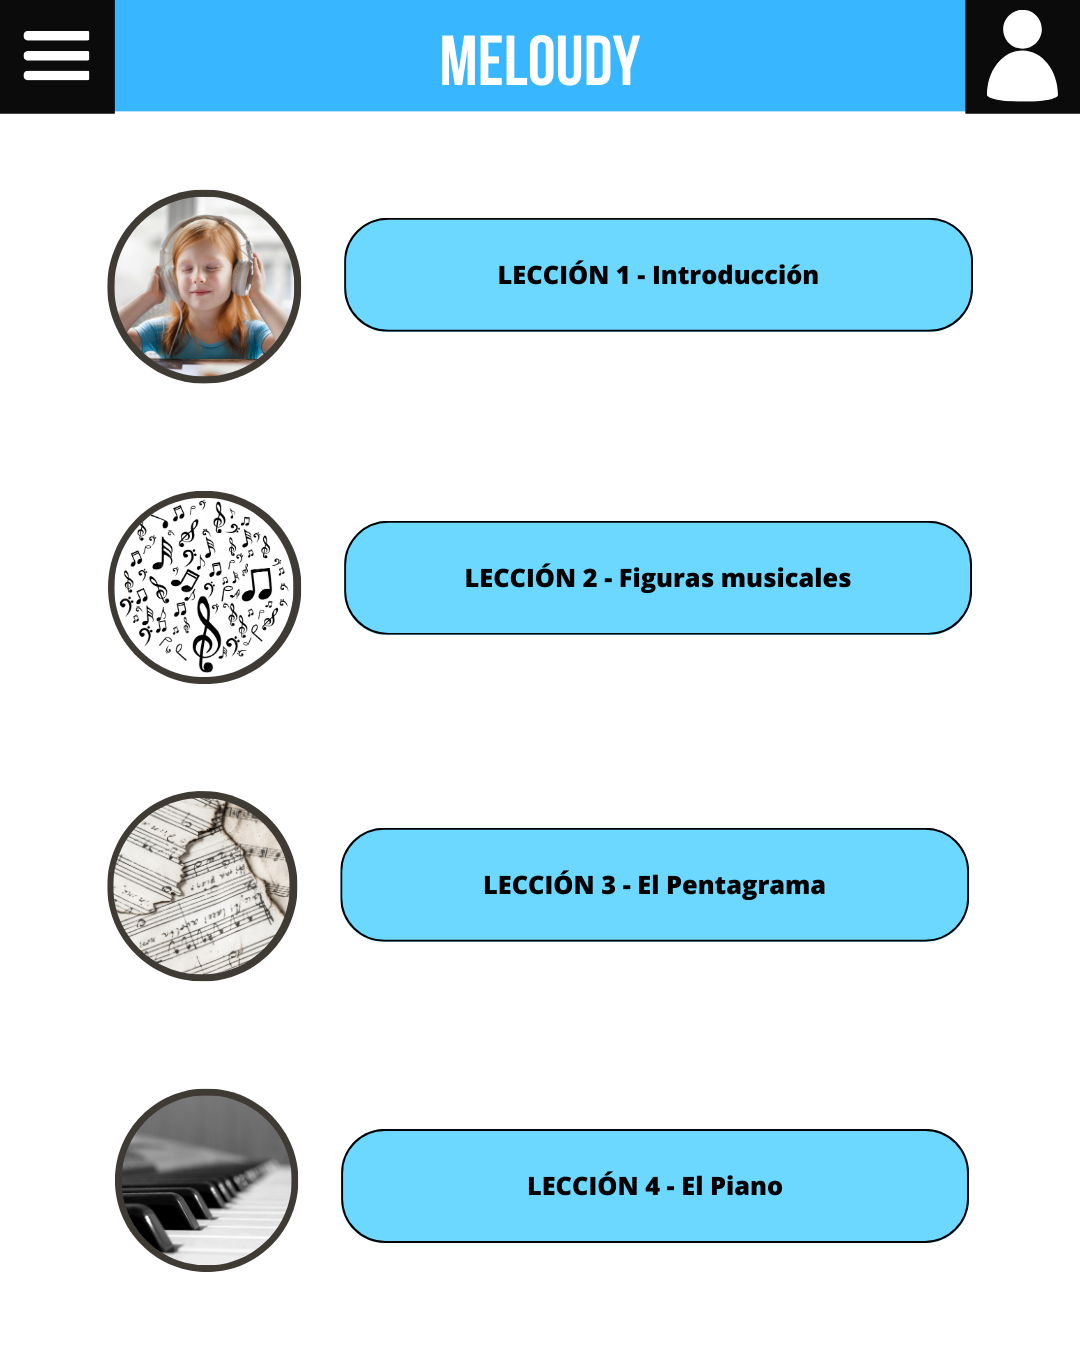
\includegraphics[width=0.55\textwidth, frame]{imagenes/c6/1.png}}
    \caption{Boceto de la pantalla principal de la aplicación donde se muestran las lecciones disponibles para el usuario.}
    \label{fig:pantallaprincipal}
    
    
\end{figure}

\begin{figure}[H]
    \centering
    \centerline{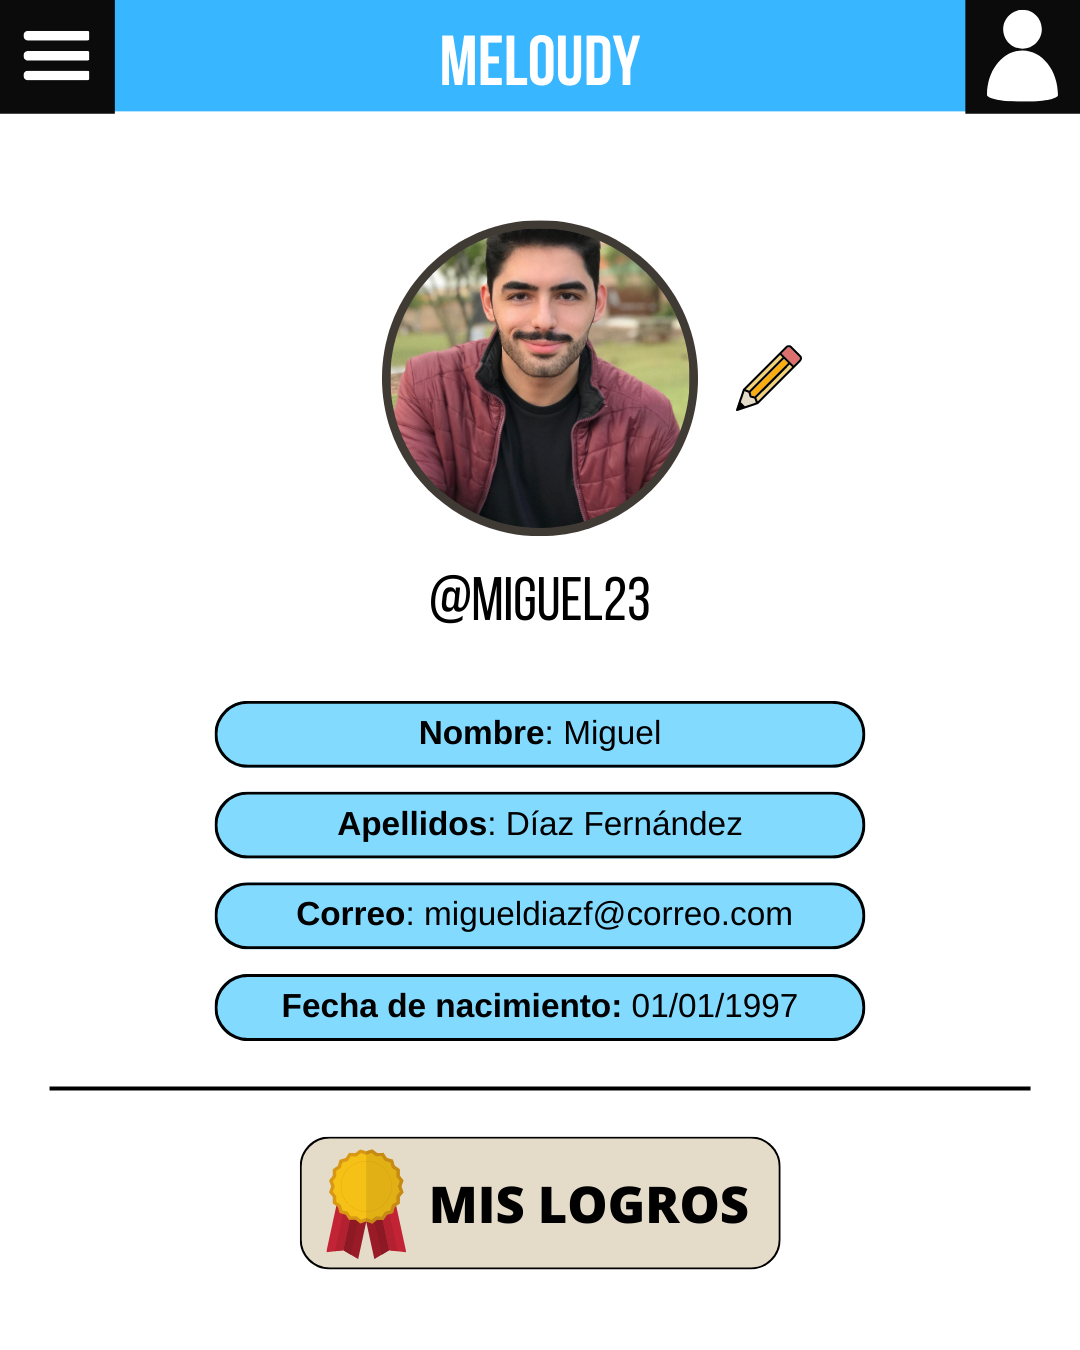
\includegraphics[width=0.55\textwidth, frame]{imagenes/c6/2.png}}
    \caption{Boceto de la pantalla del perfil de usuario con la sesión iniciada donde se muestran sus datos.}
    \label{fig:perfil}
    
    
\end{figure}


\begin{figure}[H]
    \centering
    \centerline{
\includegraphics[width=0.55\textwidth, frame]{imagenes/c6/3.png}}
    \caption{Boceto de la pantalla de logros conseguidos por el usuario.}
    \label{fig:logros}
    
    
\end{figure}


\begin{figure}[H]
    \centering
    \centerline{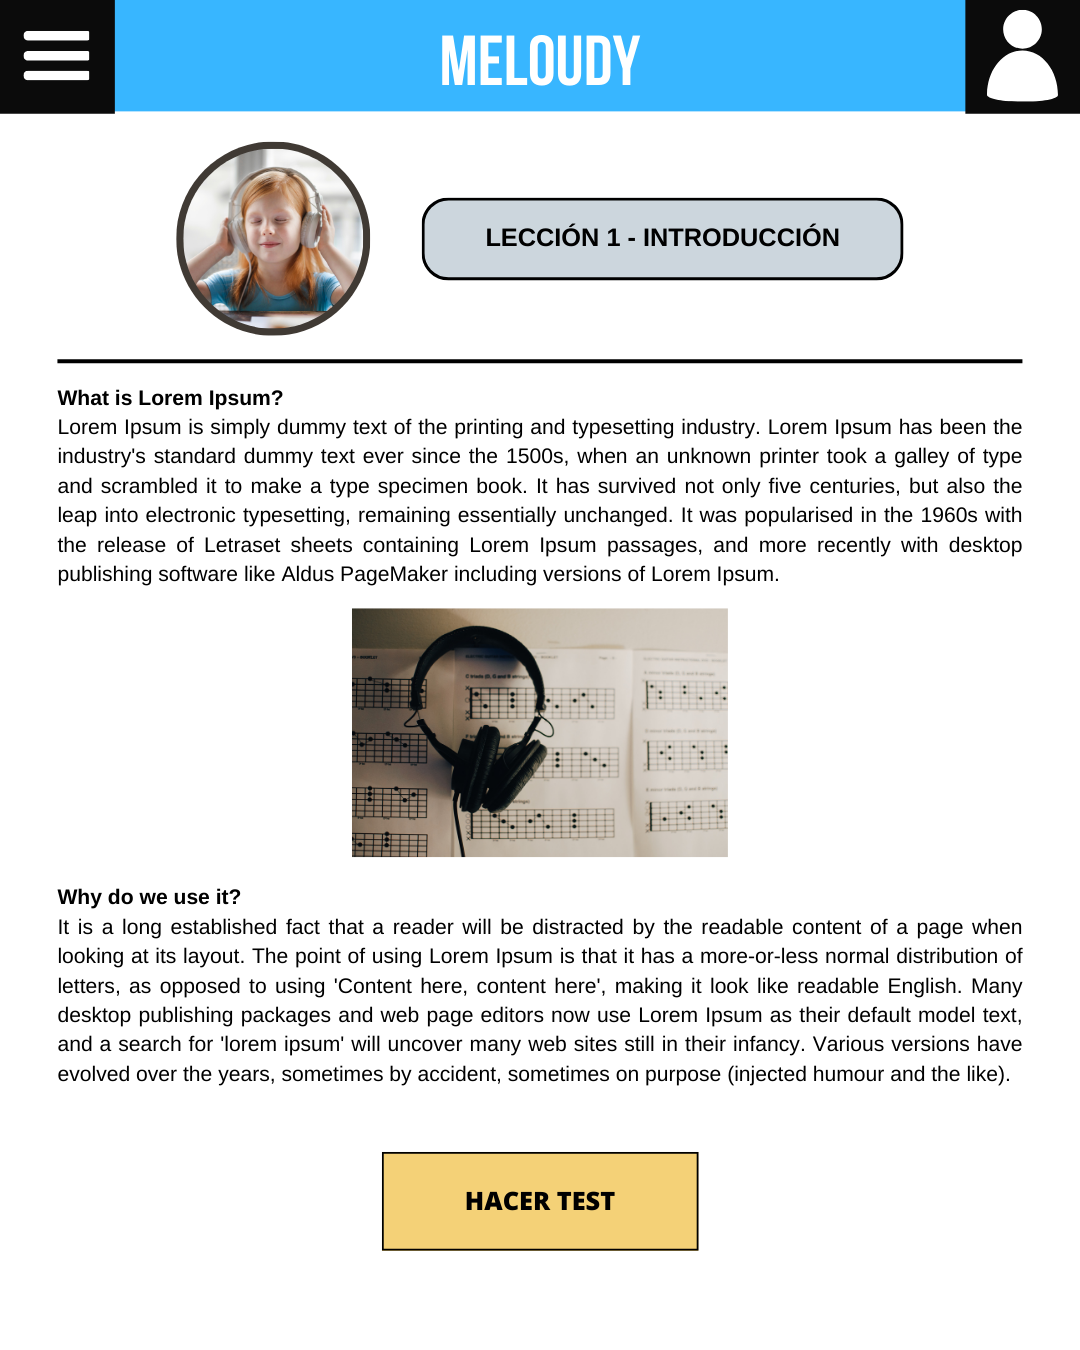
\includegraphics[width=0.55\textwidth, frame]{imagenes/c6/4.png}}
    \caption{Boceto de la pantalla de una lección, con el texto, el contenido multimedia y el botón para comenzar el test.}
    \label{fig:leccion}
\end{figure}

\begin{figure}[H]
    \centering
    \centerline{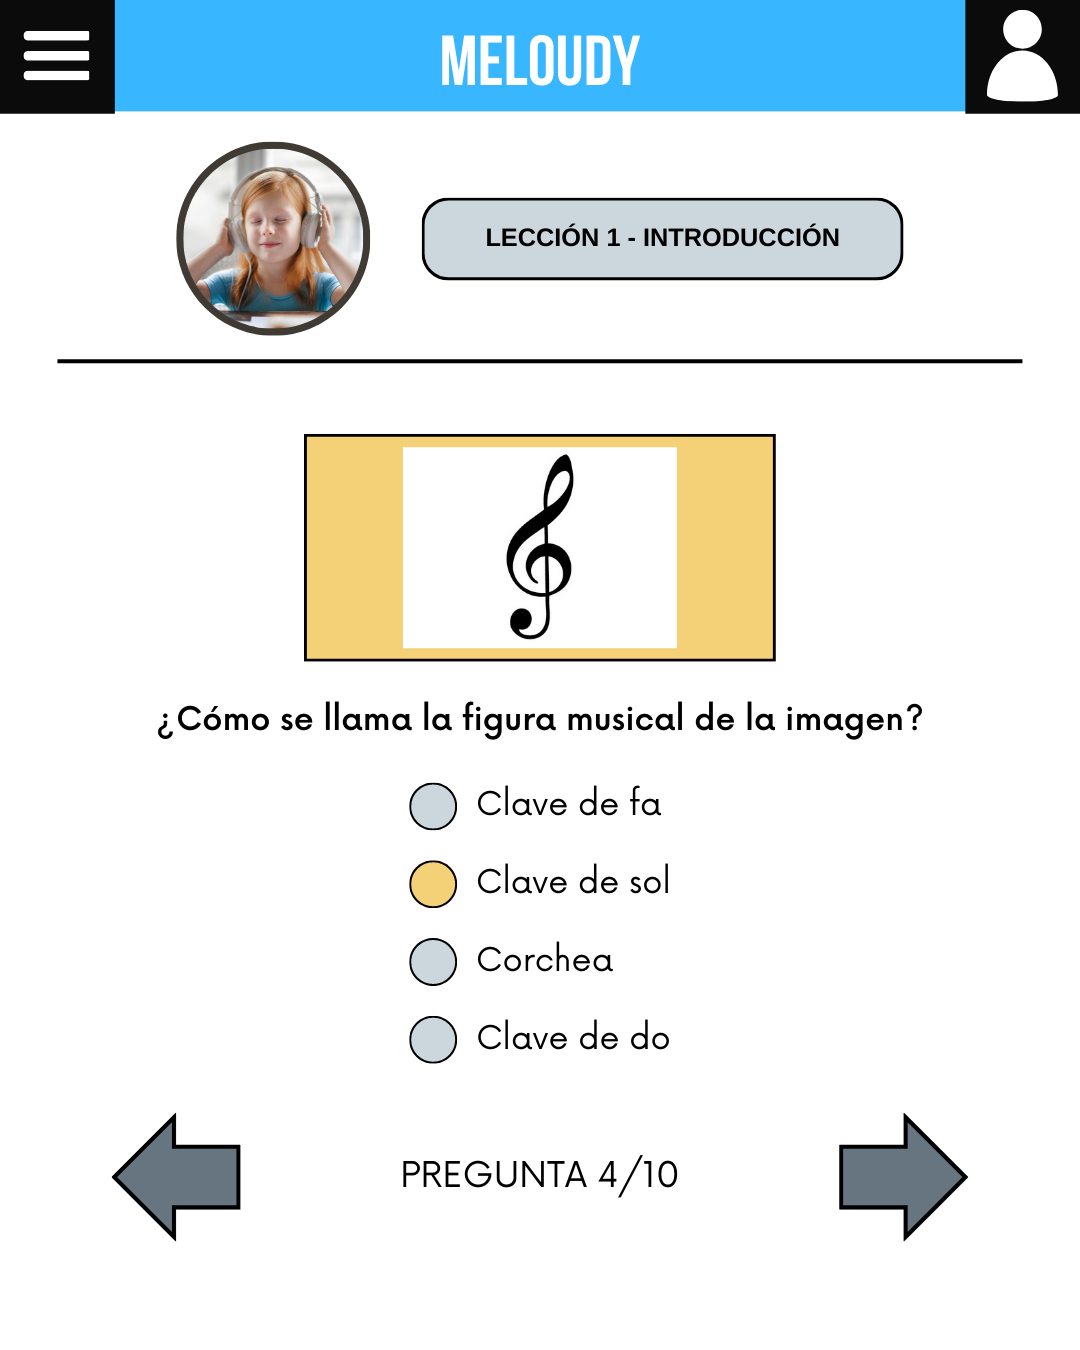
\includegraphics[width=0.55\textwidth, frame]{imagenes/c6/5.png}}
    \caption{Boceto de la pantalla de una pregunta de test de tipo selección única.}
    \label{fig:seleccionunica}
\end{figure}

\begin{figure}[H]
    \centering
    \centerline{
\includegraphics[width=0.55\textwidth, frame]{imagenes/c6/6.png}}
    \caption{Boceto de la pantalla de una pregunta de test de tipo selección multiple.}
    \label{fig:seleccionmultiple}
\end{figure}

\begin{figure}[H]
    \centering
    \centerline{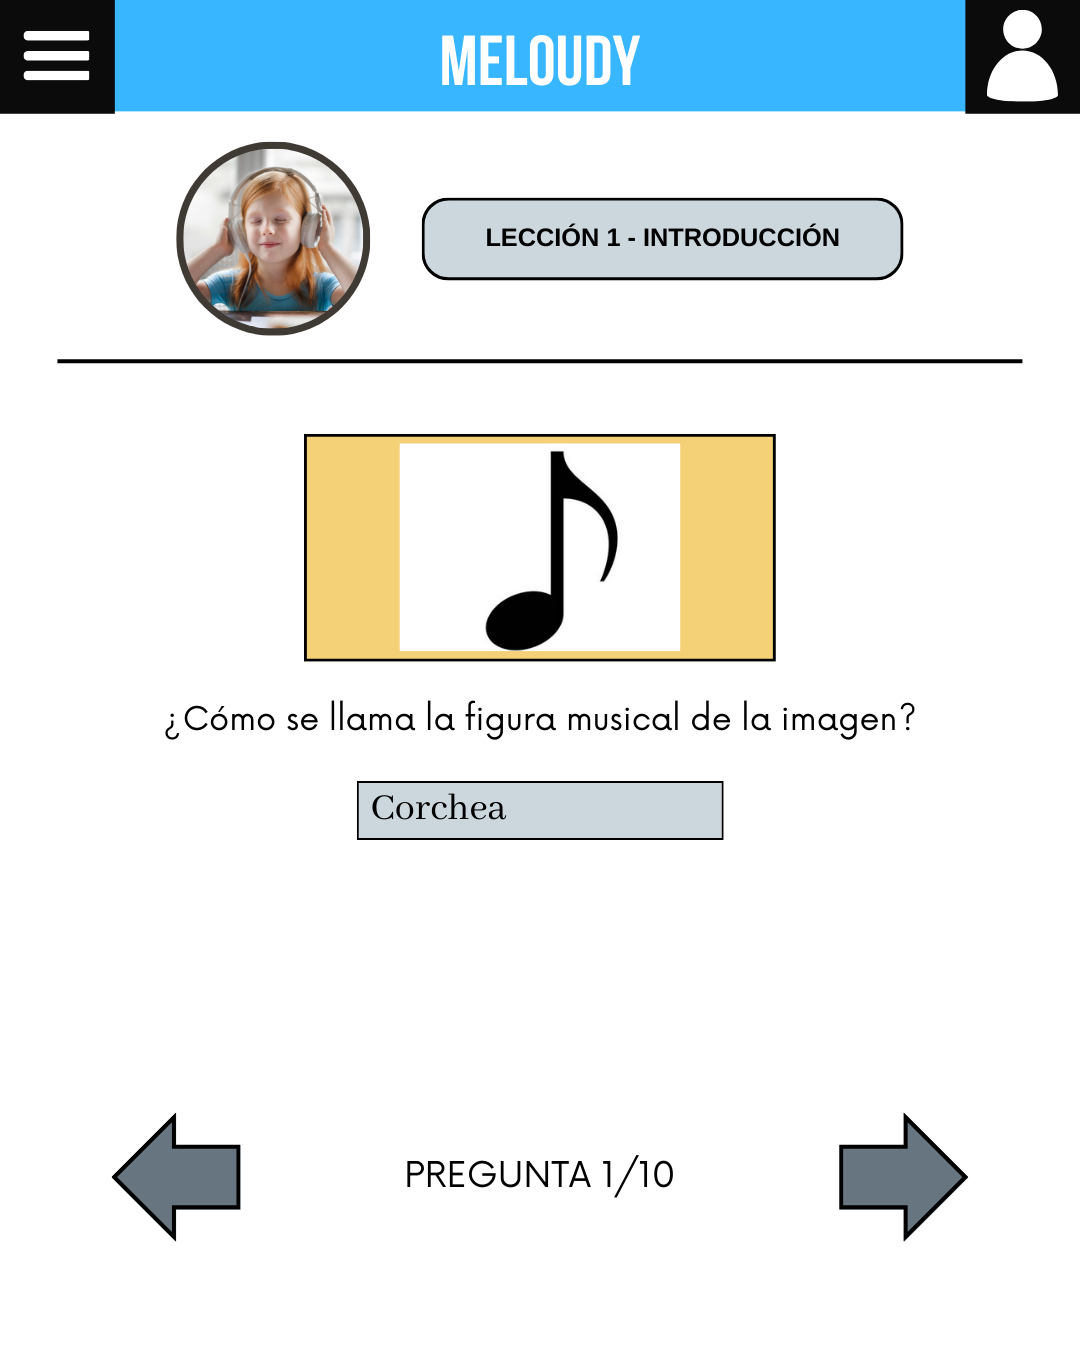
\includegraphics[width=0.55\textwidth, frame]{imagenes/c6/7.png}}
    \caption{Boceto de la pantalla de una pregunta de test de tipo escritura de texto.}
    \label{fig:escrituratexto}
\end{figure}

\begin{figure}[H]
    \centering
    \centerline{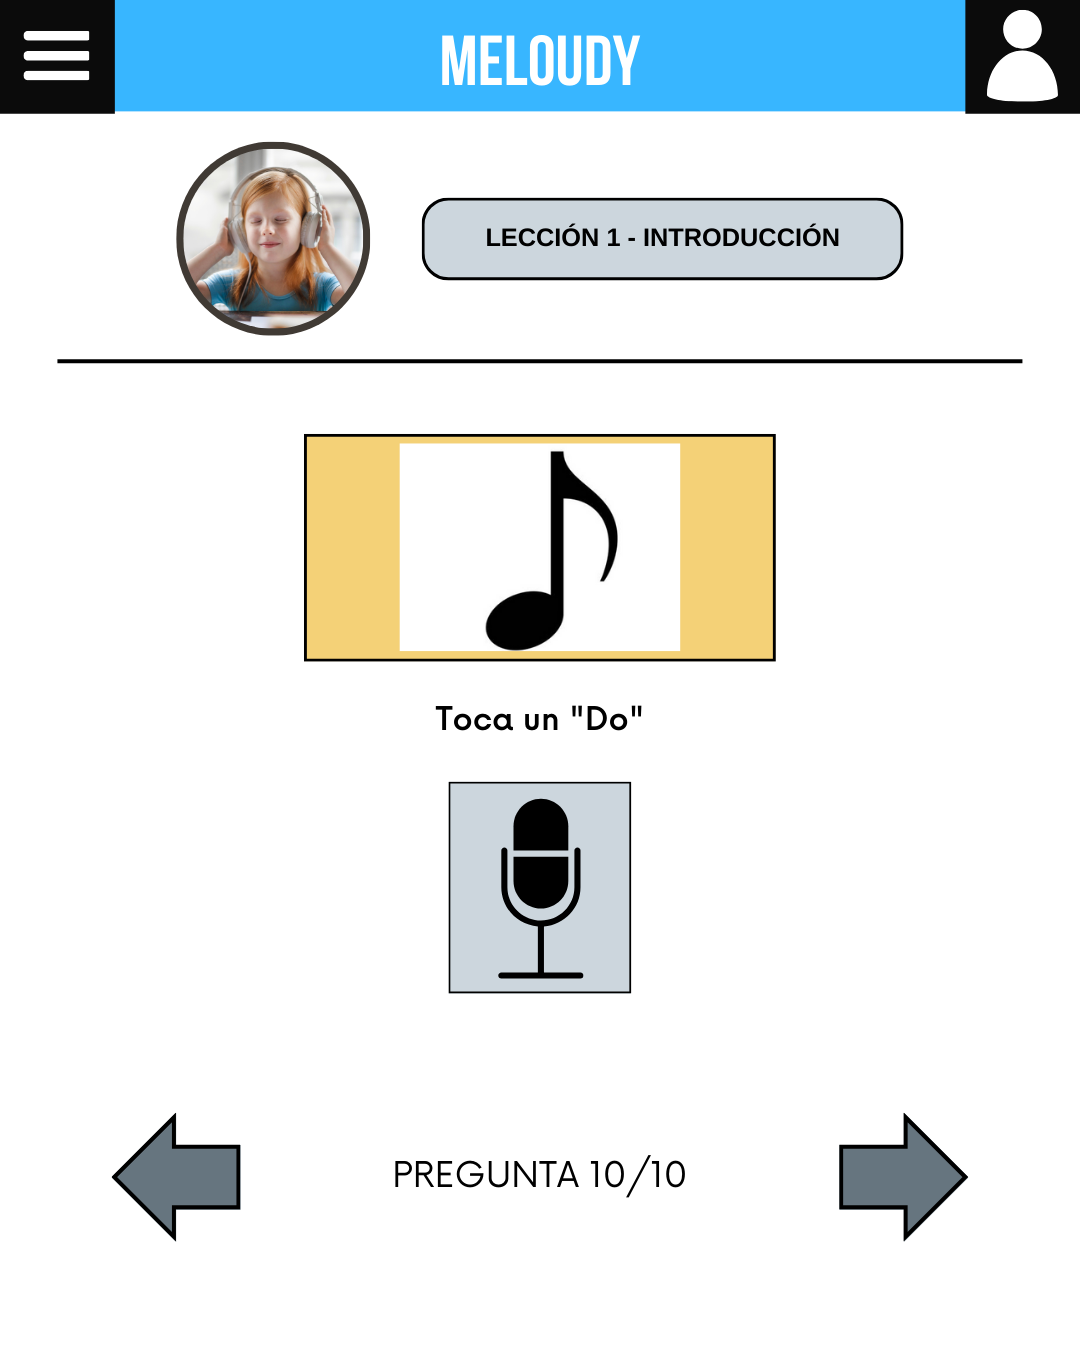
\includegraphics[width=0.55\textwidth, frame]{imagenes/c6/8.png}}
    \caption{Boceto de la pantalla de una pregunta de test de tipo entrada por micrófono.}
    \label{fig:microfono}
\end{figure}

\begin{figure}[H]
    \centering
    \centerline{
\includegraphics[width=0.55\textwidth, frame]{imagenes/c6/9.png}}
    \caption{Boceto de la pantalla de inicio de sesión, donde se pedirá al usuario el correo electrónico y la contraseña.}
    \label{fig:login}
\end{figure}

\begin{figure}[H]
    \centering
    \centerline{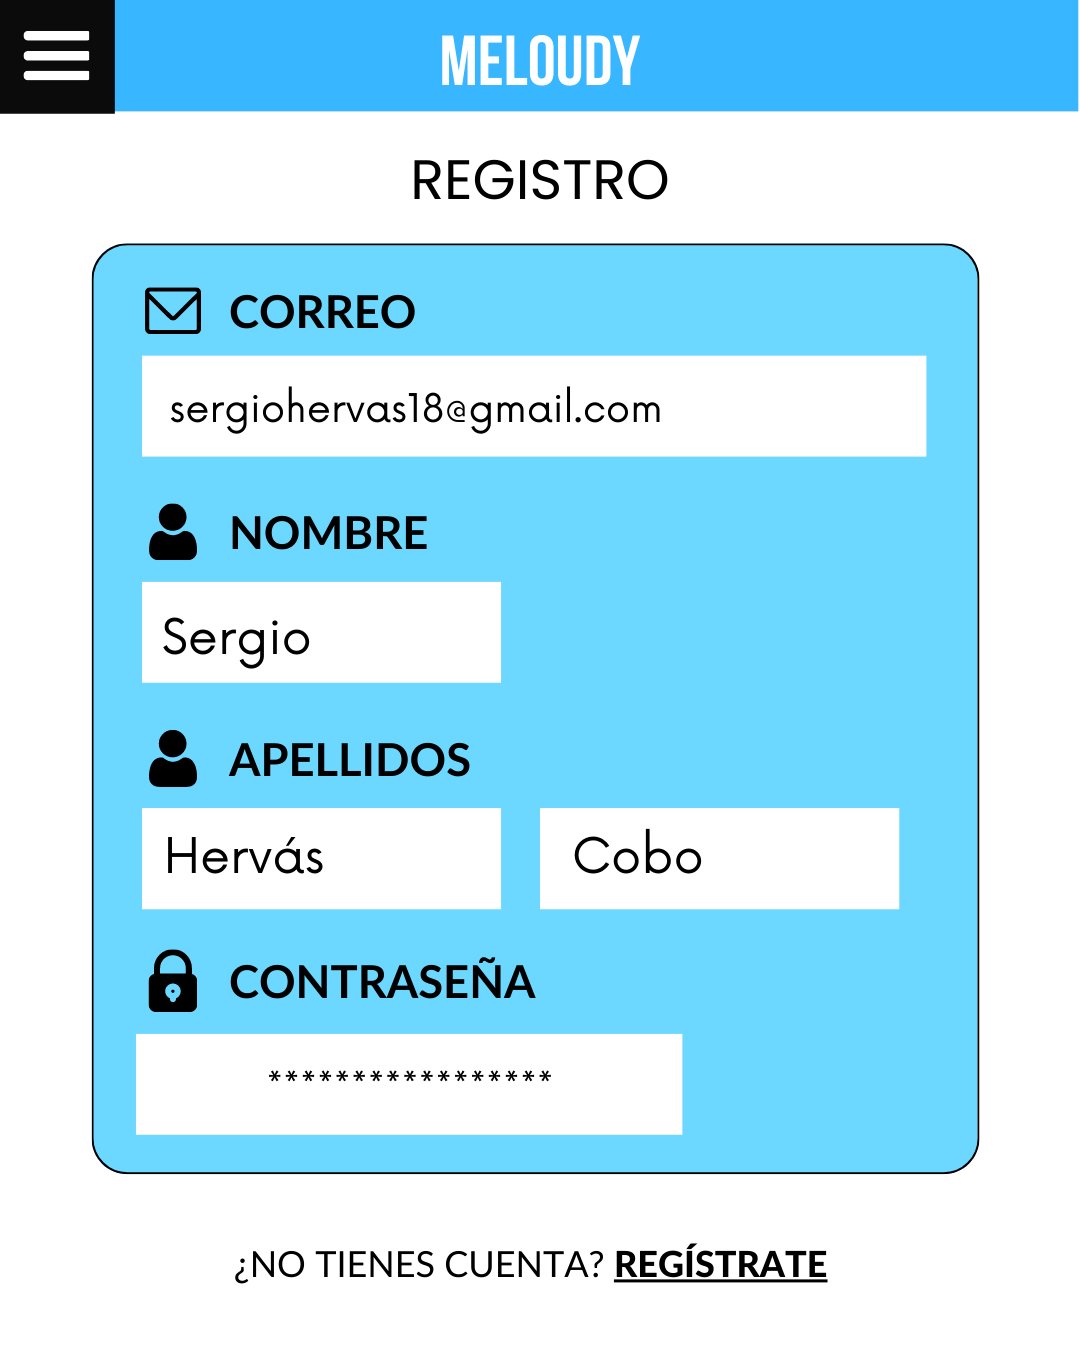
\includegraphics[width=0.55\textwidth, frame]{imagenes/c6/10.png}}
    \caption{Boceto de la pantalla de registro, donde se pedirá al usuario sus datos personales necesarios para crear la cuenta como el nombre, los apellidos, el correo y la contraseña.}
    \label{fig:registro}
\end{figure}